\documentclass{beamer}
\usetheme{Mystyle}
\begin{document}
\begin{CJK*}{UTF8}{gkai}
\begin{frame}{穿过铜片之后的能谱}
  \begin{figure}[ht]
    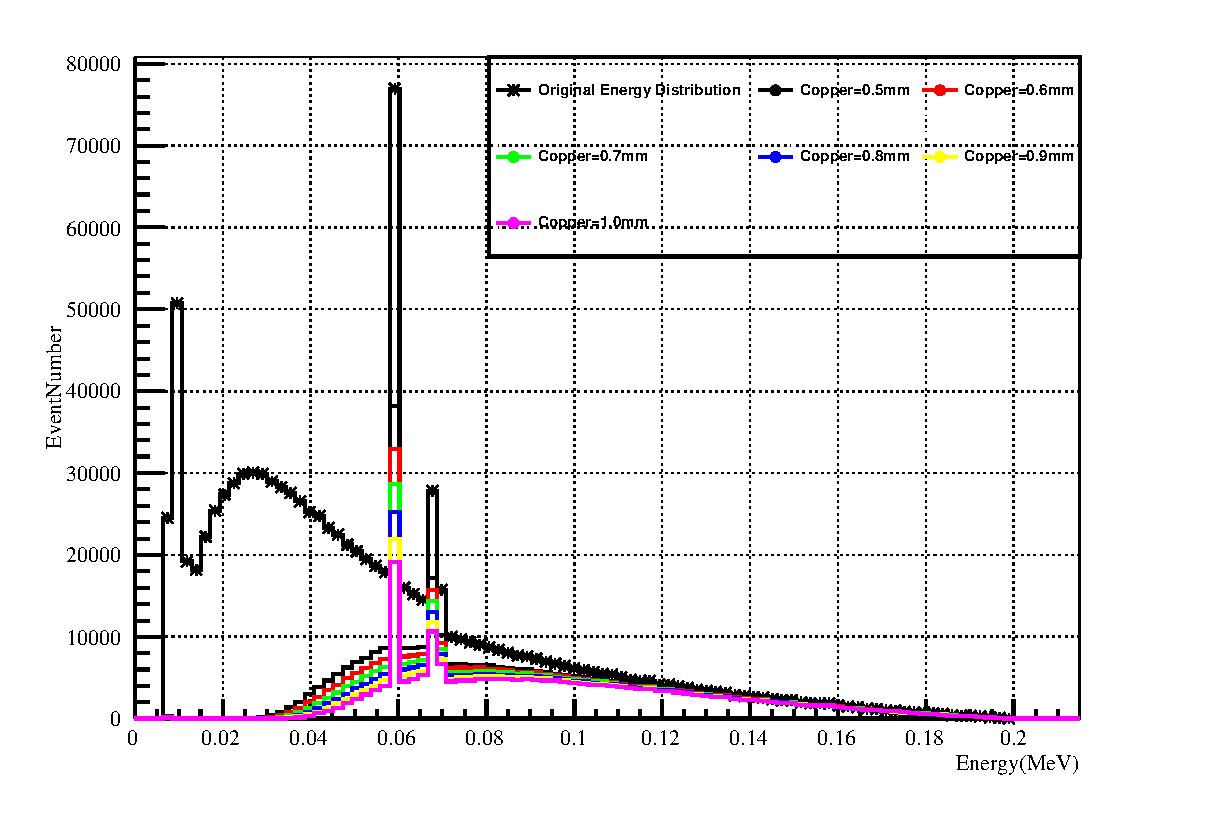
\includegraphics[width=\textwidth]{200keVEnergyAfterCopperApron.eps}
  \end{figure}
\end{frame}
\begin{frame}{穿过钛片之后的能谱}
  \begin{figure}[ht]
    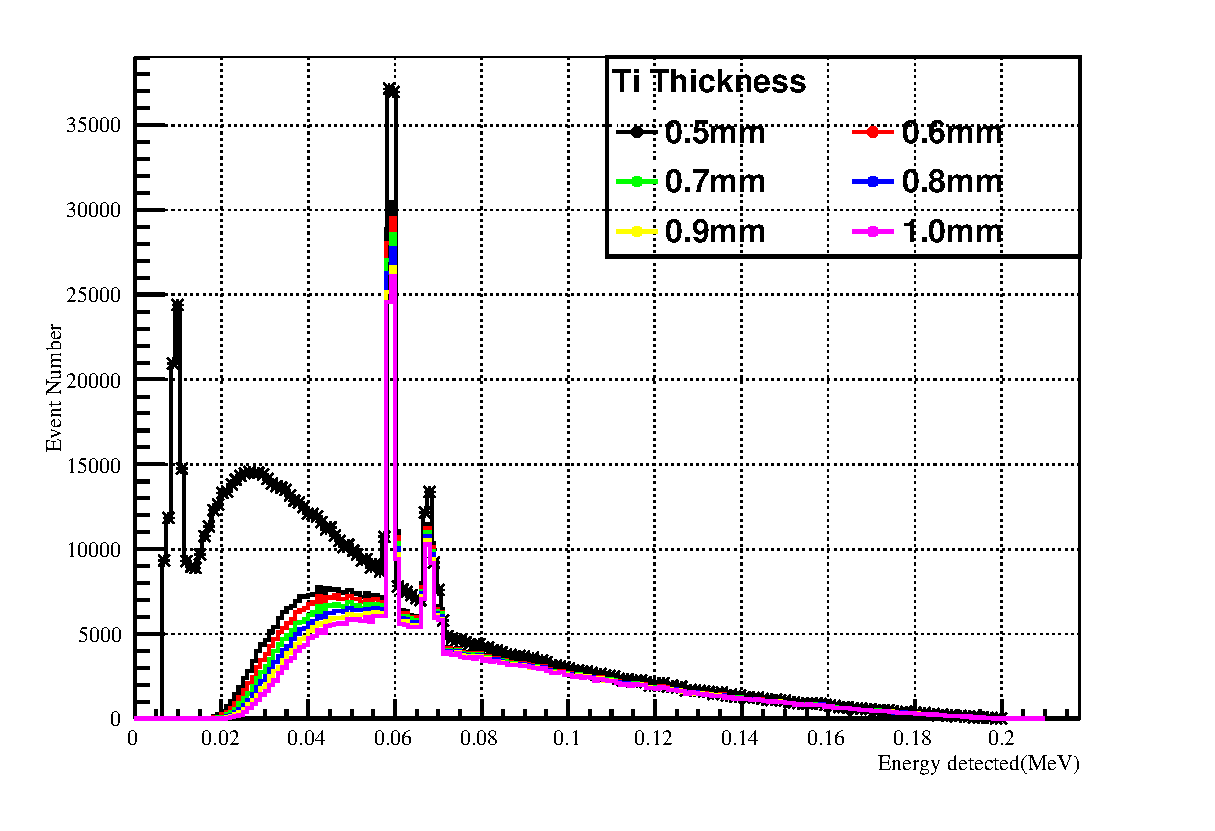
\includegraphics[width=\textwidth]{EnergyAfterTiApron.eps}
  \end{figure}
\end{frame}

\begin{frame}\frametitle{铜}
  \begin{figure}[ht]
    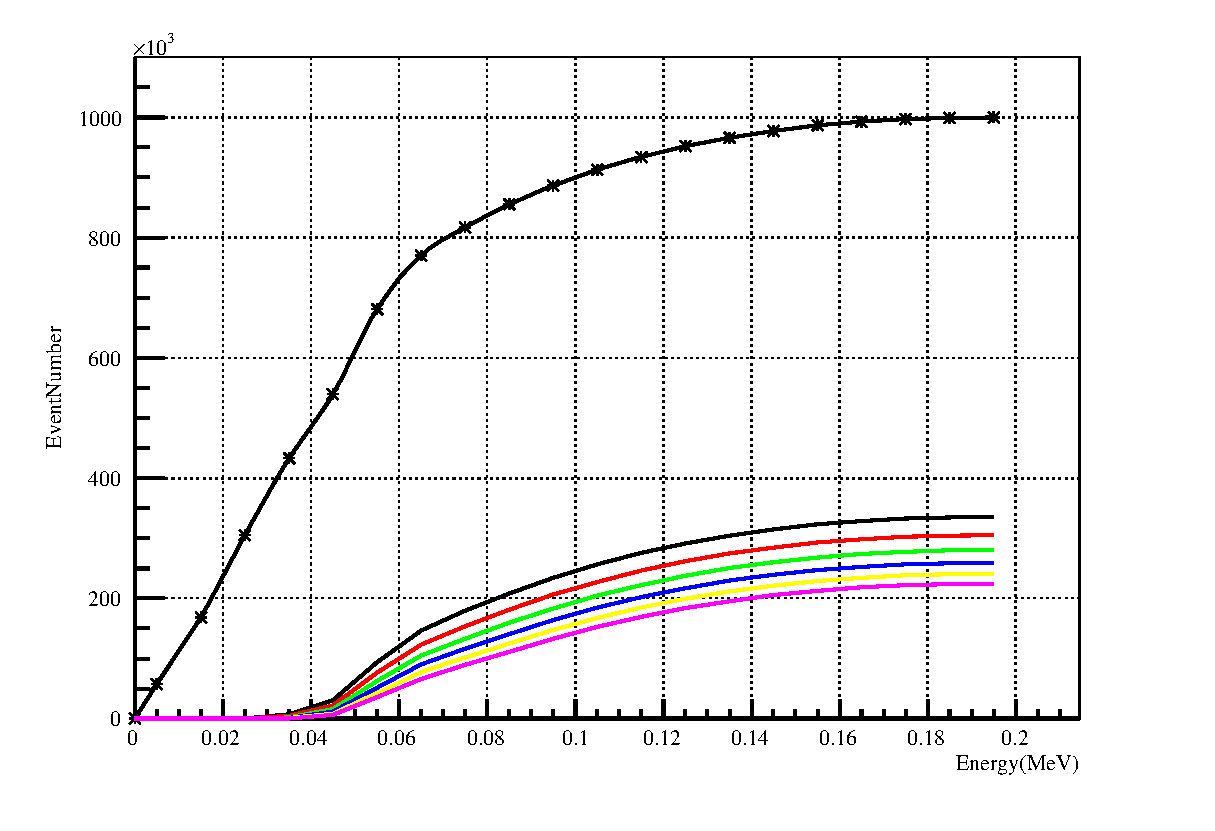
\includegraphics[width=\textwidth]{200keVElectronXrayCopperDistribution.eps}
  \end{figure}
\end{frame}
\begin{frame}\frametitle{归一化}
  \begin{figure}[ht]
    \includegraphics[width=\textwidth]{200keVElectronXrayCopperDistributionRatio.eps}
  \end{figure}
\end{frame}
\begin{frame}\frametitle{钛}
  \begin{figure}[ht]
    \includegraphics[width=\textwidth]{200keVElectronXrayTiDistribution.eps}
  \end{figure}
\end{frame}
\begin{frame}\frametitle{归一化}
  \begin{figure}[ht]
    \includegraphics[width=\textwidth]{200keVElectronXrayTiDistributionRatio.eps}
  \end{figure}
\end{frame}

\end{CJK*}
\end{document}
